\chapter{Test of the final system}\label{ap:final_test_report}

To make the final test of the drone, the control system has been program for the Teensy on the drone, and the  system has been tested in the motion tracking lab.

As discussed in section \ref{sec:control_code}, the drone has to be manually flown to the point where it hovers. Here the pilot flips a switch to set the gravity offset thrust, and set the initial set-point. If the operator flips the switch to the next position, 100 mm is added to the set point.

This was the procedure used in the motion tracking lab, and the drone was tracked using the Vicon system to track its height over time. Additionally code was added that tracked the demanded throttle every 20ms, and once the aforementioned switch was returned to it's initial position, would save the last 20 seconds of these samples to EEPROM on the micro-controller. This would then be output on power-up over serial, when the drone was connected to a PC.

The resulting height data and throttle data can be seen on figure \ref{fig:first_test}

\begin{figure}[H]
    \centering
    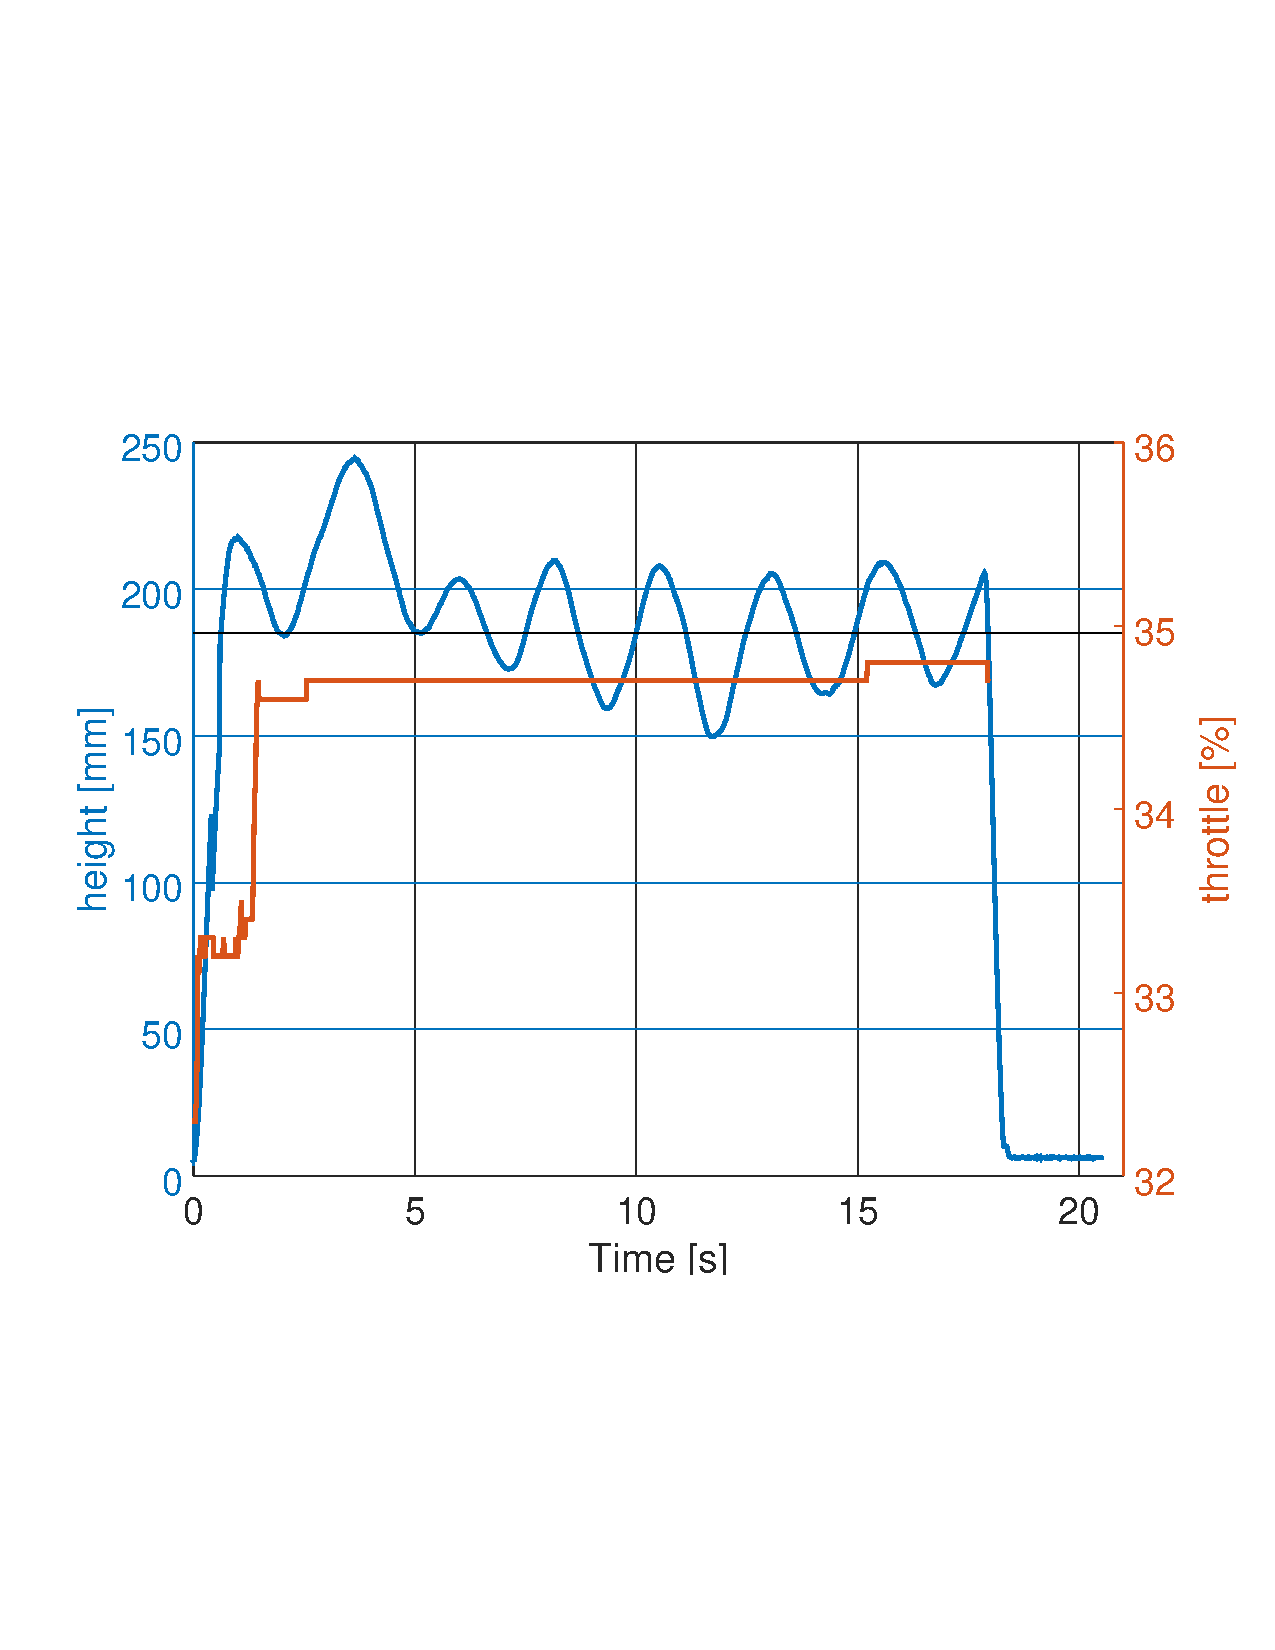
\includegraphics[width=0.9\textwidth, trim={0 7cm 0 7cm},clip]{figures/Appendix/final_test/kp0,012.pdf}
    \caption{Height graph Kp = 0.012. Marker line is at 185 mm}
    \label{fig:first_test}
\end{figure}

From this first test, it was clear that our gain was too low, as the regulator only produced a maximum output swing of 0.1\% throttle over the gravity offset. because of this we tuned the gain from 0.012 to 0.05, and performed a second test. The result of this test can be seen on figure \ref{fig:second_test}.
With this test, we still didn't see the expected result from the regulator, so we further increased Kp to 0.1 and discovered a new problem.

\begin{figure}[H]
    \centering
    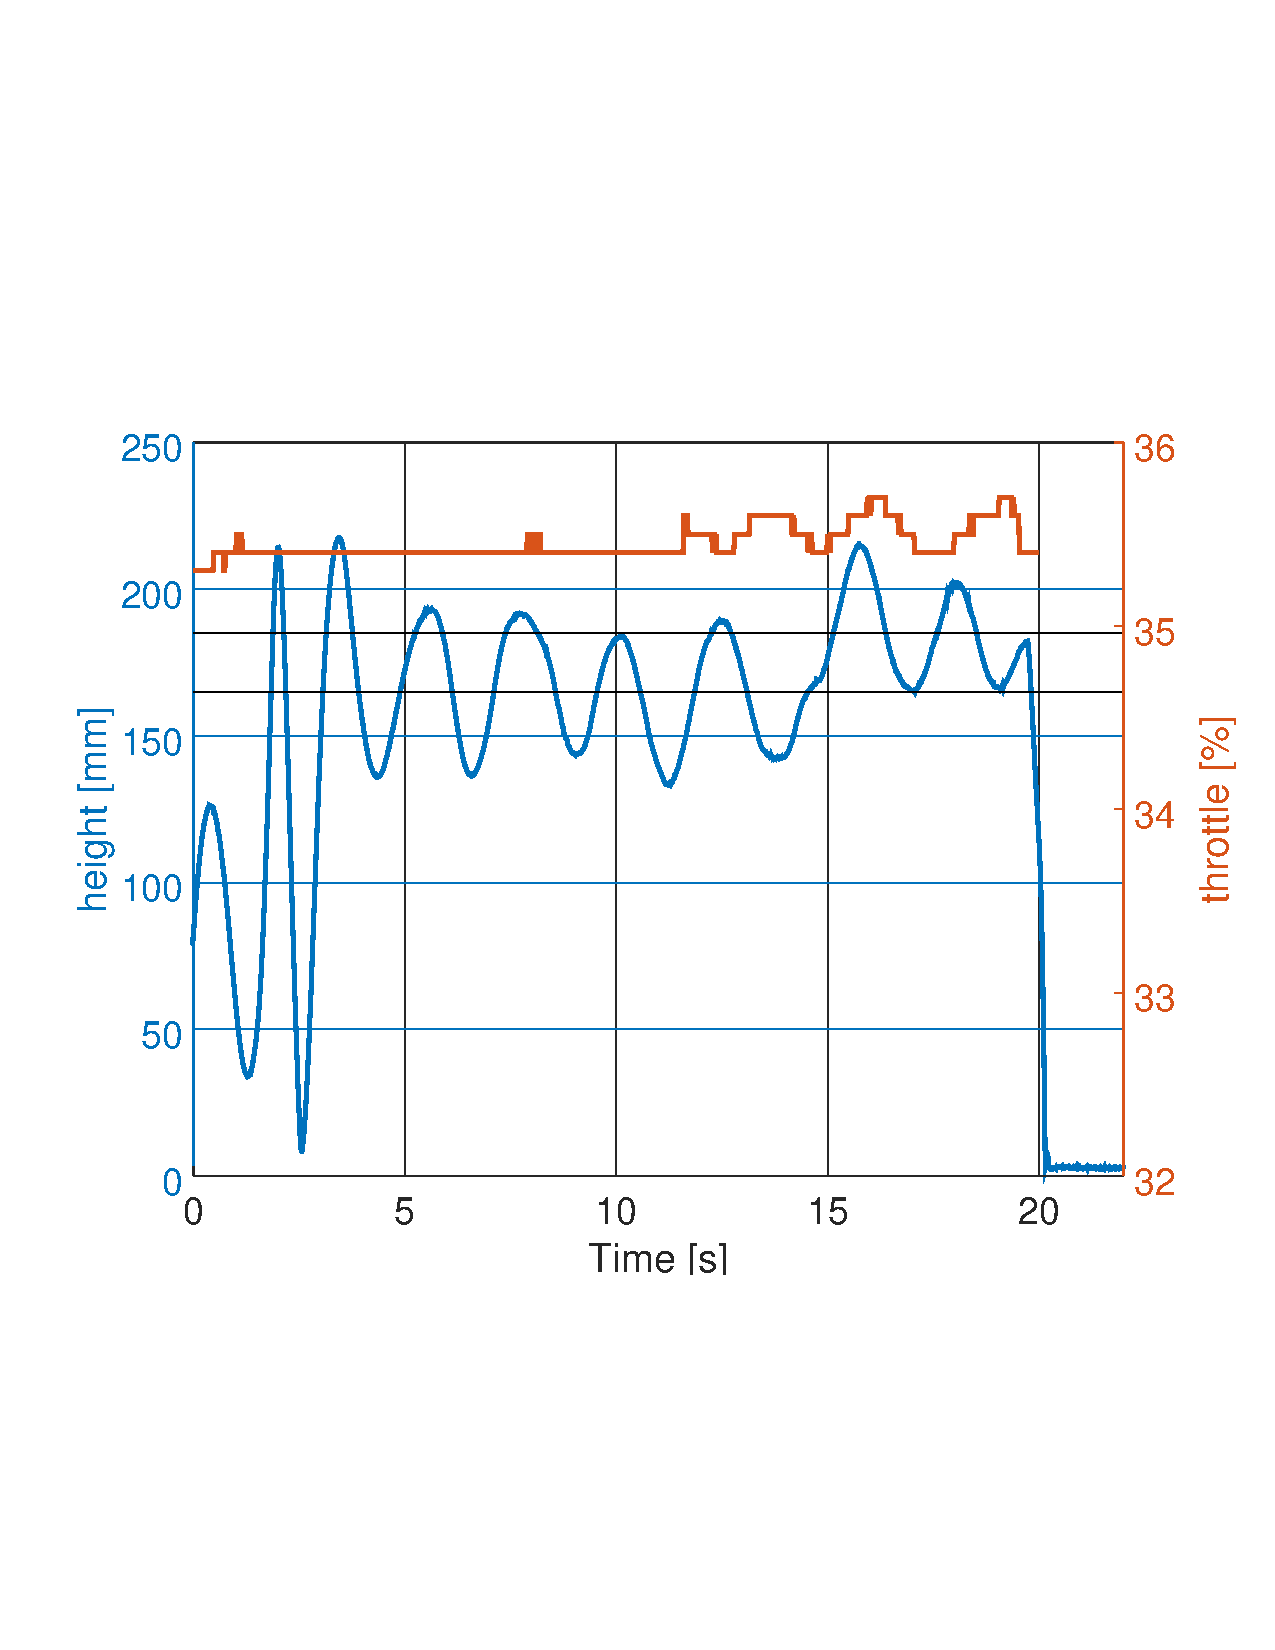
\includegraphics[width=0.9\textwidth, trim={0 7cm 0 7cm},clip]{figures/Appendix/final_test/kp0,05.pdf}
    \caption{Height graph Kp = 0.05. Marker lines are at 165 and 185 mm}
    \label{fig:second_test}
\end{figure}

\begin{figure}[h]
    \centering
    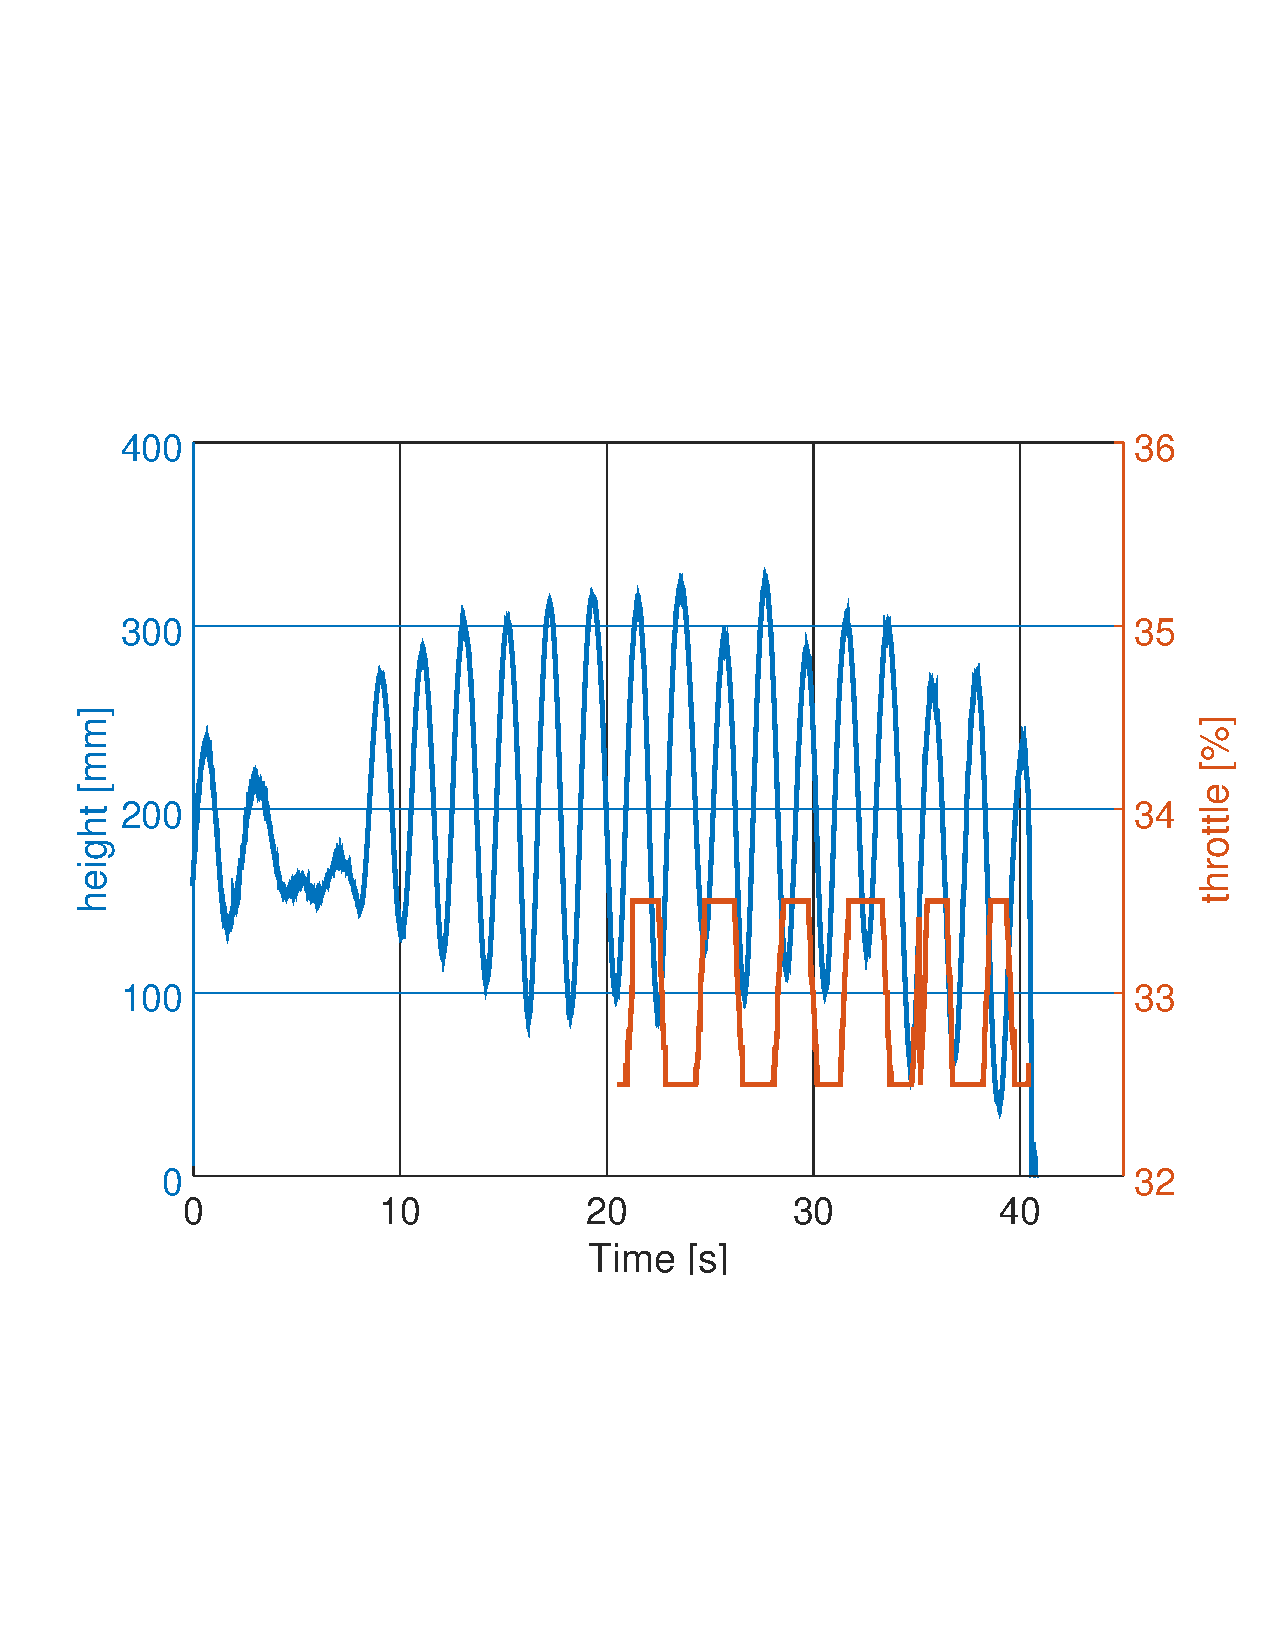
\includegraphics[width=0.9\textwidth, trim={0 7cm 0 7cm},clip]{figures/Appendix/final_test/kp0,1.pdf}
    \caption{Height graph Kp = 0.1.}
    \label{fig:third_test}
\end{figure}

\begin{figure}[h]
    \centering
    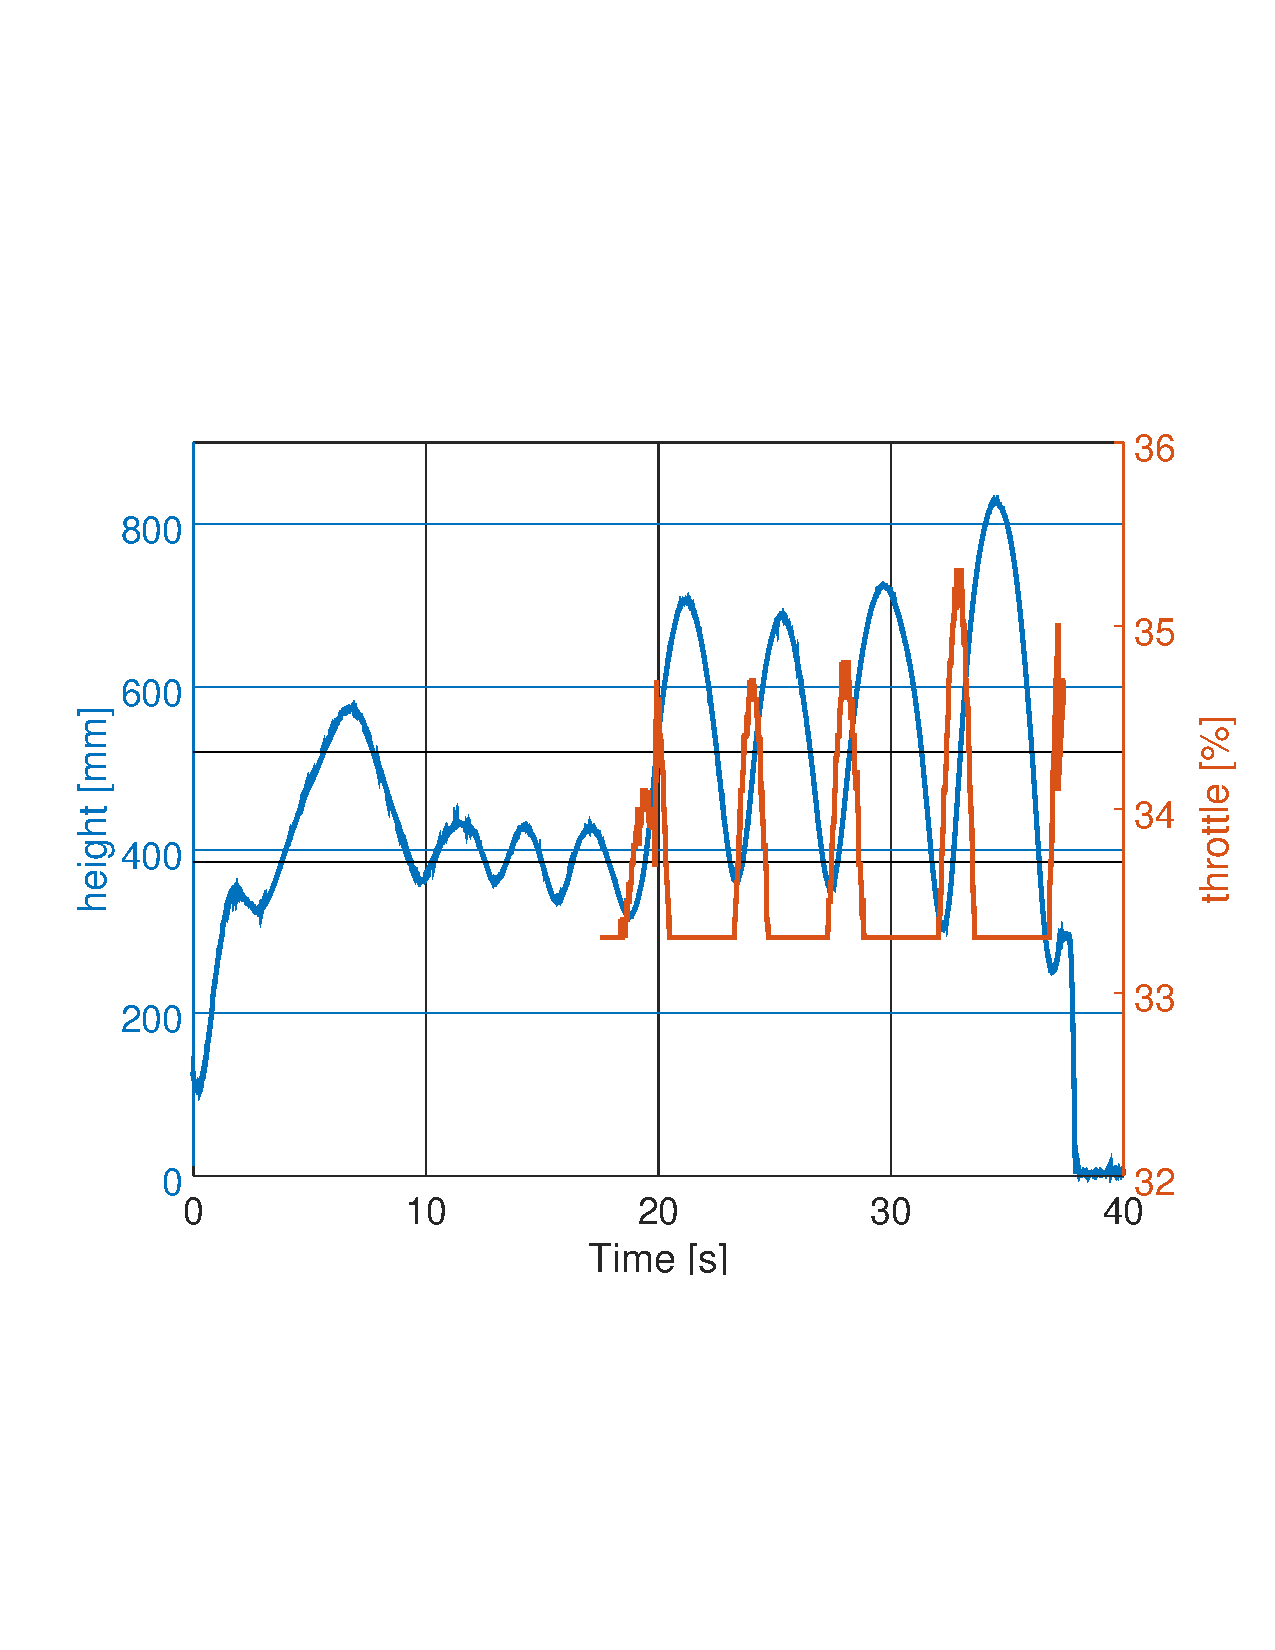
\includegraphics[width=0.9\textwidth, trim={0 7cm 0 7cm},clip]{figures/Appendix/final_test/kp0,1fix.pdf}
    \caption{Height graph Kp = 0.1 with fixed saturation. Marker lines are at 385 and 520 mm}
    \label{fig:fourth_test}
\end{figure}


The regulator is limited in code to saturate early in order to avoid an improperly tuned regulator from crashing the drone, as full throttle is far too high for our drone, and especially for use inside. However the new Kp highlighted a problem with this limiting, as seen on figure \ref{fig:third_test}. The limiting was supposed to be 10\%, but as the code works in steps of 0.1\% it was mistakenly set to 1\% This was corrected, and the behaviour seen on figure \ref{fig:fourth_test} was observed. In this test we achieved closer to what we had expected, but we do see significant oscillations, and high overshoot.